\chapter{Introduction} \label{chap:introduction}
Hook paragraph; work in progress.
Main points will be:
Earth is vast;
Earth is diverse;
Earth is important (home to all of humanity/all life).
Therefore, important to understand the Earth so we can make informed decisions regarding it.

%Yet despite the cosmic insignificance of the Earth, all of humanity---and in fact all life we are aware of---call this planet home. From the [] of the [] to the [] of the [], the Earth is both vast and diverse. Given that Earth is the [], humanity has collected large amounts of data the planet.  Likewise, the data available about the Earth is similarly vast and diverse. 

%Given its significance to all of humanity, it is vital to understand and protect the Earth.

One of the ways humanity works toward better understanding the Earth is by gathering data about it.
Remote sensing satellites and aircraft, along with various smart technologies, have created a significant increase in the amount of geospatial data available and continually being collected.
This has led to the challenge of \textit{geospatial big data}, meaning that the volume and complexity of data exceed the capacity of current computing systems~\cite{lee2015geospatial}.
With applications in urban planning, agriculture, education, natural disaster prediction and management, and many other fields, the development of technologies for managing geospatial data is more crucial than ever.
These tools are needed to efficiently integrate, process, analyze, and visualize geospatial data in order to use it to make informed decisions.
Such a need has led to the vision of Digital Earth, where all data regarding the Earth is available in a common reference used by the public to inform their decisions.
The use of such a system would range from world governments informing policy by analyzing climate trends to homeowners referencing local utility line locations when building a fence.
In reality, such an expansive and holistic system is yet to be achieved; however, many approaches for smaller-scale Digital Earths exist.


Geographic information systems (GIS) are one of the conventional approaches used for creating a Digital Earth.
With a GIS, different datasets are represented and stored as individual map layers in a planar coordinate system, which acts as a proxy for the Earth.
These individual layers are overlayed to create a complete model of the Earth (or region of the Earth) and combined with different operations to perform various analyses.
However, being created and gathered by diverse organizations, geospatial data exists in many different formats and resolutions.
The conventional GIS pipeline---which requires experts to clean, process, integrate, and distribute data---is unsustainable in the face of geospatial big data.
Furthermore, even after data has been integrated with a GIS, overlay operations such as intersections and data extraction are computationally expensive when many data layers are present~\cite{wang2015improving}.
Coordinate based representations of geospatial data also do not provide proper facilities to represent the uncertainty or error of the data they are used to represent. [goodchilde reimagine]


Another challenge with GIS is the use of a flat map as the underlying representation.
Flattening the Earth produces inevitable map edges and distortion that impact the analysis and visualization of geospatial data.
Map edges can cause serious misunderstanding of the continuity between different sides of the map---especially with young children~\cite{hennerdal2015beyond}---and also affect the estimation of distance even when the continuity is correctly understood~\cite{hruby2016journey}.
Distortion causes inaccuracies in calculations such as geodesics and buffering if planar geometry is used~\cite{flaterbuffering}, which is especially problematic when working with large distances and areas.
These distortions also affect the visual analysis of data by misrepresenting the size and shape of different regions.


Model globes avoid many of the shortcomings of planar maps by providing a more accurate reference model for the Earth.
Despite this, the ability for physical maps to be easily made and stored, display the entire Earth at once, and accommodate any scale has made them the preferred option in many situations.
With the advent of a Digital Earth, however, many the drawbacks of physical globes are lessened or negated.
Computer graphics algorithms and hardware allow globes to be rendered in real-time, storage is no different than for a digital map, and interactive systems allow zooming and panning to show any part of the Earth at any scale.
The only challenge unsolved is displaying the entire Earth at once; however, even this is partially addressed with multi-view focus plus context rendering techniques~\cite{mark-sherlock}.
Because of this, there has been a recent push toward globe based Digital Earth systems, one of the most well-known examples of which being Google Earth\footnote{url here}.
In these systems, data is visualized on a 3D model of the Earth---approximated as a sphere or ellipsoid---as opposed to a traditional planar map. While globe based Digital Earths are becoming more popular, many of these systems still use a flat map as the underlying representation for geospatial data.
Thus, these systems still suffer errors introduced by distortion resulting from any planar operations done with the underlying coordinate system.


A common approach to avoid coordinate-based representations of geospatial data is to use an area- or cell-based representation.
A partition of the Earth into a set of non-overlapping cells allows information to be associated with the cells(s) that correspond with the appropriate region(s) of the Earth.
Such partitionings are termed discrete global grids (DGG).
To accommodate different resolutions of data, a hierarchy of these DGG's at successively finer resolutions, referred to as a discrete global grid system (DGGS), is used.
Not only does this cell hierarchy allow multiple resolutions of data to be supported, but it also provides an inbuilt mechanism for representing data uncertainty by using a cell (or set of cells) to represents the range of possible locations for a datum.
However, in order for DGGS cells to serve as a suitable representation for geospatial data, these cells should be compact and near-uniform in size.
Compact cells ensure that data from geographically distant (relative to the size of the cell) locations are not represented in the same cell.
Uniformity of size ensures that each resolution of the DGGS represents the entire Earth at a particular spatial resolution and that cells of the same size do not appear at different resolutions of the grid system.


While DGGS's are an effective tool for integrating and managing geospatial data on the surface of the Earth, they have no inbuilt mechanism for supporting 3D data.
Many of today's geospatial sensors, along with other technologies such a numerical weather prediction, generate data with an associated altitude in addition to other dimensions.
With a DGGS, 3D data is flattened with altitude stored only as an attribute.
This has motivated the development of volumetric (3D) discrete global grids and grid systems to allow native support for 3D data.
Going forward, we use the term 3D DGGS to refer to these technologies collectively.


Most human activity and interest, and correspondingly geospatial data, is located in a relatively small region above and below the surface of the Earth ($\pm$10 -- 500 km).
Likewise, most existing approaches for 3D DGGS's have focused on this region.
However, there are select processes such as seismic wave propagation and the magnetosphere that span much beyond this region (\textbf{figure?}).
Furthermore, the range of altitudes satellites orbit at is extensive, with satellites in high Earth orbit exceeding 36,000 km.
Therefore, to support the full range of human activity and interest, 3D DGGS's that extend to the centre of the Earth and far beyond the atmosphere are needed.


\section{Problem Statement}
Despite the necessity for 3D DGGS's, the area of research is still relatively unexplored compared to that of traditional DGGS and GIS technologies.
Additionally, of the proposed methods, many are only appropriate for data with small altitude ranges, or data near the surface of the Earth.
Thus, for data with more extensive altitude ranges, there are even fewer methods that are appropriate. 
From this, we arrive at the primary goal of this thesis: to develop 3D DGGS's that have adequate support for unbounded ranges of altitude. 


A simple approach for such a 3D DGGS would be to embed the Earth in a 3D Euclidean voxel partitioning or similar space partitioning data structure, for which many efficient and well-tested algorithms exist.
While such a system is simple in its construction, it ignores the spherical nature of the Earth.
Cells are not aligned with the surface of the Earth, which means there is no consistent orientation of up (increasing altitude) and down (decreasing altitude) with respect to a cell.
Likewise, traversal along the surface of the Earth is complex and requires ``zig-zagging'' up and down.
This type of grid also provides a poor approximation for the surface of the Earth, especially at low resolutions.
While these issues are negligible for small scale regions of the Earth, for a 3D DGGS with global coverage, the underlying grid should be sphere-based and Earth-centric.
Cells should be aligned with the surface of the Earth and have a consistent orientation for increasing and decreasing altitude.


\begin{figure}[tb]
	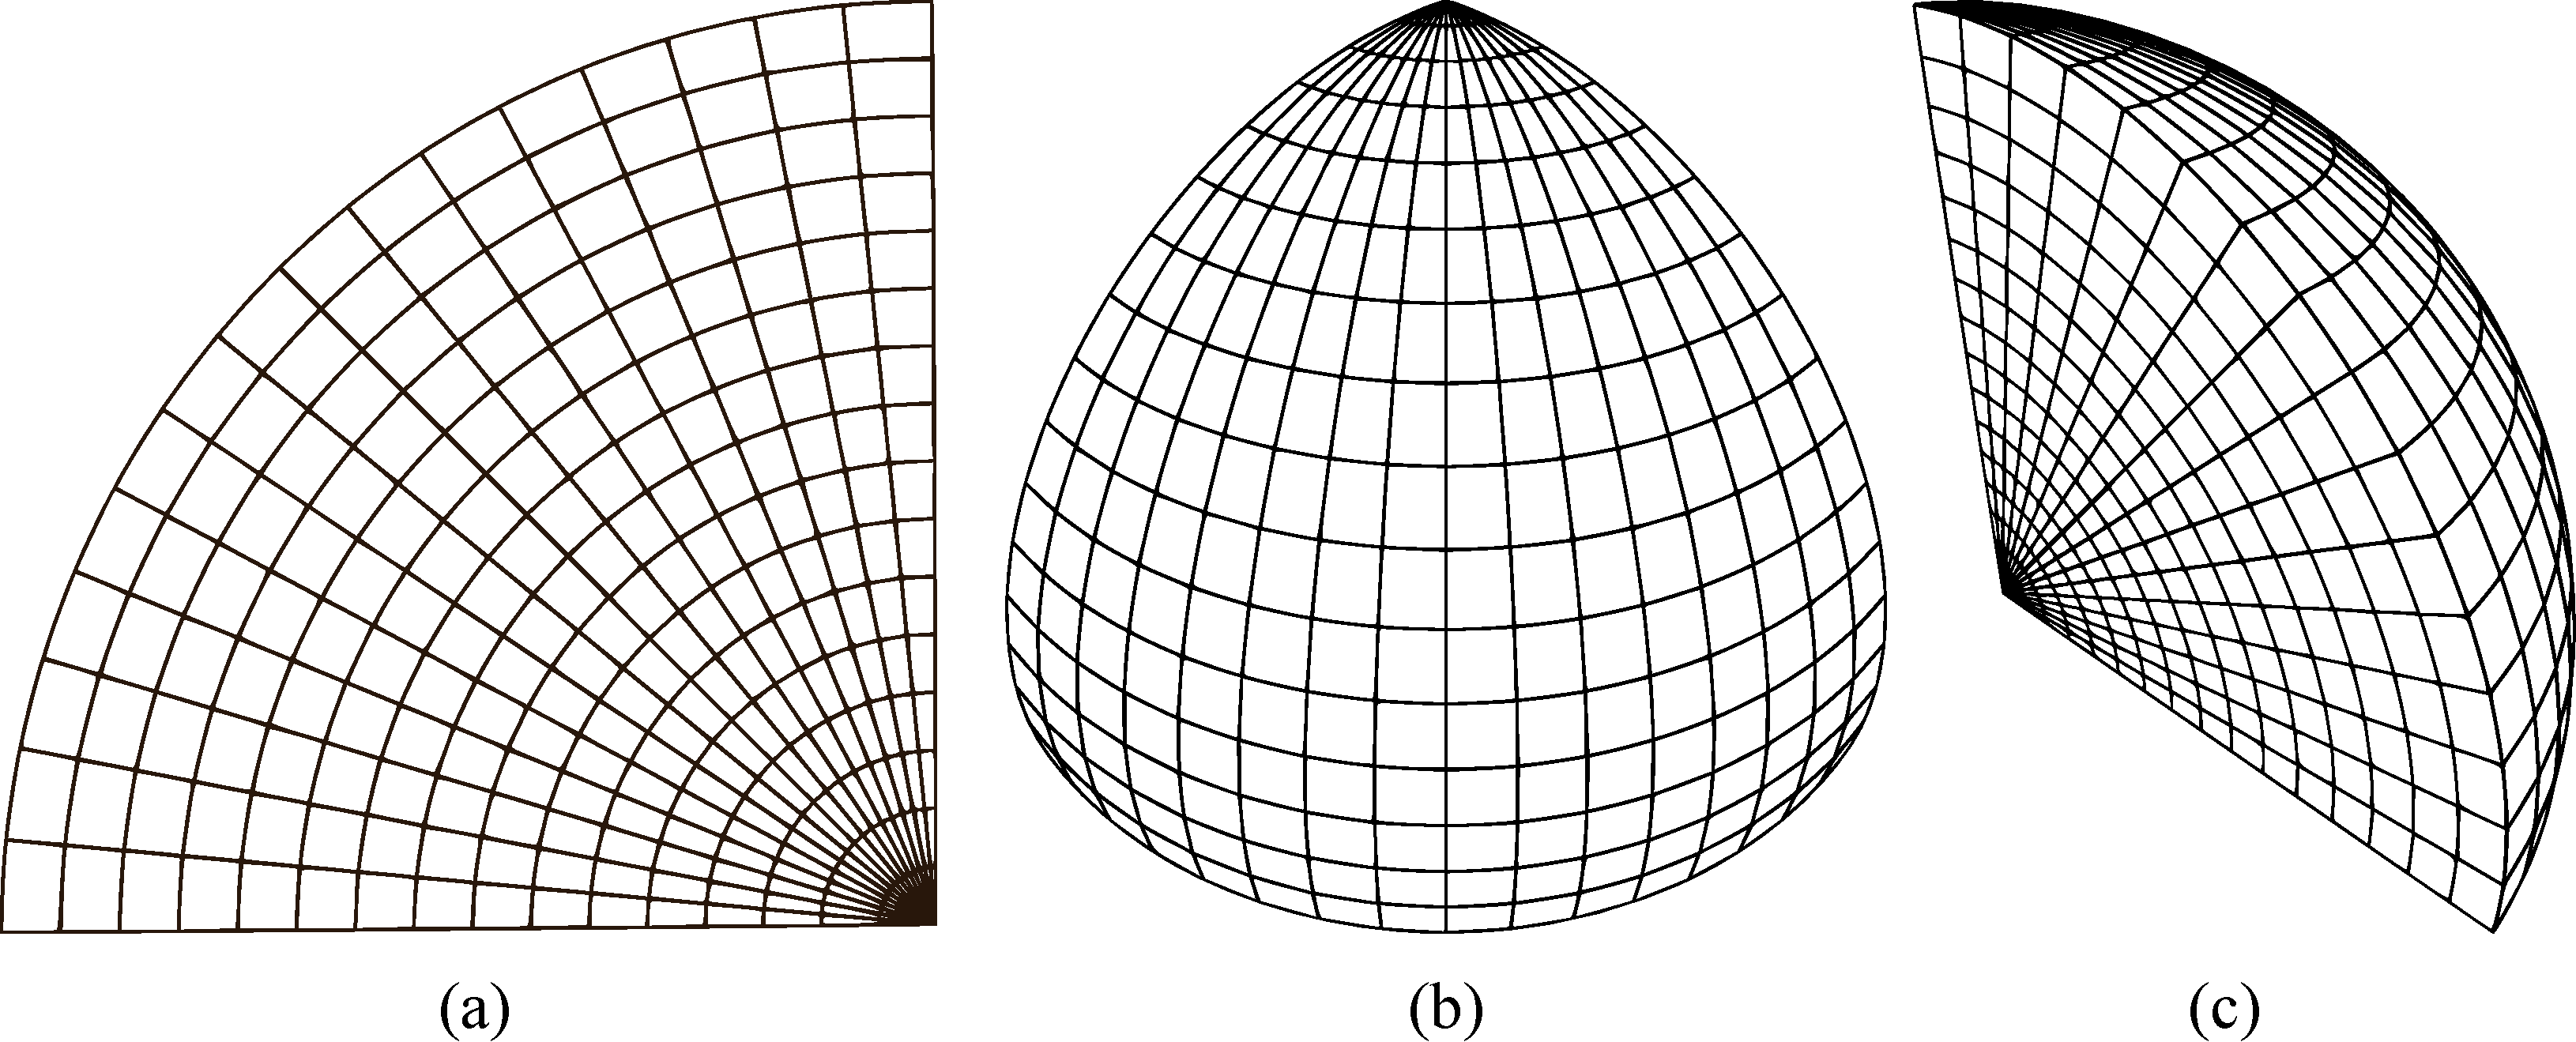
\includegraphics[width=\textwidth]{Fig1.pdf}
	\caption[Different Views of a 3D Latitude-Longitude Grid]{
		placeholder figure.
		Caption describing degeneration in cells toward centre and poles
	}
	\label{fig:3dllg}
\end{figure}


The main challenge associated with such Earth-centric grids is the inevitable degeneration of cells toward the singularity at the centre of the Earth.
This effect is demonstrated in Figure~\ref{fig:3dllg}---cells more near the centre of the grid become increasingly small and skinny and eventually degenerate to pyramids.
For grids with a small radial extent, the effect of this is negligible; however, for the range of altitudes we wish to support in this thesis, it cannot be ignored.
The problem with this type of cell degeneration is two-fold, as it reduces both the compactness and volume of cells. 
Furthermore, the resulting difference in the volumes of cells is unbounded.
It is worth noting that this same issue presents itself in traditional latitude-longitude grids at the poles, also demonstrated in Figure~\ref{fig:3dllg}.
Addressing such cell degeneration is one of the main challenges of this thesis.


\section{Goals and Scope}
In addition to the initial goal of supporting an unbounded range of altitudes, there are several other aims for a 3D DGGS we wish to explore in this thesis.
While we discuss these below in the context of a 3D DGGS, they are equally applicable to their conventional 2D counterparts.
We choose to explore these goals only for Earth-centric 3D DGGS's using semiregular degenerate refinement strategies (see chapter 3.something); limiting the scope in this manner allows a more thorough exploration of the goals in the 3D DGGS's we propose.


As discussed previously, the cells of a 3D DGGS need to be compact while also maintaining near-uniform volume.
Ideally, all cells of the grid would be exactly congruent; however, with an Earth Centric grid, this is impossible.
Therefore, for our 3D DGGS's, we aim to have cells with similar shapes and sizes without sacrificing compactness.
In addition to near-uniform volume, cells being \textit{exactly} equal volume is beneficial in specific applications.
Calculating the volume of a cell can be an expensive operation, which significantly impacts the speed of analysis if this property is needed frequently.
If all cells have the same size, this calculation is replaced with a constant resulting in a significant performance increase in these applications.
Thus, we also aim to have perfectly equal volume cells in our 3D DGGS's when it is possible and desired to do so.


Once the cells of a 3D DGGS are defined, methods for mapping geospatial data to the appropriate set of cells are needed.
Likewise, the inverse process of mapping data associated with a set of cells back to the corresponding regions of the Earth is needed for visualizing data on the globe.
These two operations are referred to as grid encoding and grid decoding (or just encoding and decoding), respectively, and allow the integration of geospatial data with the grid system.
With data integrated, analyses such as region growing and data aggregation require spatial neighbourhood and hierarchy traversal queries.
Ensuring all these operations are efficient allows quick integration, processing, analysis, and visualization of data with the 3D DGGS.


Finally, our 3D DGGS should leverage the accomplishments already made with conventional DGGS to facilitate the efficient and straightforward transference of data between 2D and 3D DGGS's. This interoperability allows smooth migration from 2D to 3D systems while also providing backwards compatibility from 3D to 2D systems.


Given these goals and scope, we refine the goal of this thesis: develop methods for Earth-centric 3D DGGS's using semiregular degenerate refinement to support unbounded ranges of altitude, equal (or near-equal) volume cells, efficient operations, and interoperability with 2D DGGS's.


\section{Methodology}
In this thesis, we use two different approaches to create 3D DGGS's with the desired properties.
The first approach modifies the refinement rules of an existing 3D DGGS, the Spheroid Degenerated-Octree Grid (SDOG)~\cite{yu2009sdog}, to improve its volume-preserving properties.
With SDOG, a sphere with twice the radius of the Earth is initially divided into eight equal octants via the equatorial plane and two perpendicular meridian planes.
Cells (including the initial octants) are then refined using splitting surfaces located at the midpoint of the three spherical coordinates: latitude, longitude, and radius.
To prevent cell degeneration near the poles and centre of the grid, the extent of splitting surfaces (and the number of resulting children cells) depends on the shape of the cell that is being refined.
We perform the modifications by analyzing the placement of these splitting surfaces and finding ideal new locations that result in cells of the most uniform volume possible given certain constraints.


The second approach is a general method for creating a 3D DGGS that uses a conventional polyhedron based DGGS as a starting point and specification.
First, we create the initial 3D discretization by extruding the faces of the initial polyhedron of the input DGGS into prismatoid cells.
Bases of prismatoid cells are then refined using the same refinement scheme as the input DGGS and combined with a radial refinement.
Such an approach for creating a 3D DGGS allows the research, development, and data integration achieved with conventional DGGS to readily be leveraged with the 3D one.
We take care to perform the extension in such a way that it achieves the desired properties of the 3D DGGS regardless of the 2D one used.
The extension also allows for an additional property, a target aspect ratio for cells, to be attained.


For both of these approaches, we define mappings between physical points and their corresponding locations in grid space, which are used to implement efficient encoding and decoding operations.
For the SDOG based approach, we provide constant time encoding and decoding algorithms that outperform the standard versions of these algorithms at high levels of refinement.
These new algorithms can be used both with conventional SDOG and, by using the provided mappings, the volume-preserving one.
We also provide similar algorithms for the 3D DGGS's that result from the extension method.


We evaluate the effectiveness of the first approach using two metrics of volume preservation: one for the maximum difference in volumes and one for the distribution.
We also use a third metric to evaluate the impact these modifications have on the compactness of cells.
For our proposed encoding and decoding algorithms, we compare the runtime performance with the conventional algorithms at different levels of refinement both for conventional SDOG and our modified grids.


Evaluation of the second approach is done through a series of use cases, each employing a different combination of input DGGS and 3D parameters to create a resulting 3D DGGS most appropriate for the application.
These use cases illustrate both the versatility and sophistication of the method, being able to quickly create many different 3D DGGS's while achieving the desirable properties outlined above.


\section{Contribution}
This main contributions of this thesis fall into three groups:

\begin{enumerate}
	\item Modifications of SDOG refinement.
	These modifications are able to achieve perfect volume preservation between all non-degenerate cells.
	Additionally, we provide blending functions that allow a balanced trade-off between volume preservation and cell compactness.
	An analysis of volume preservation and compactness for the different modifications is also provided.
	
	\item Method for extending 2D DGGS to 3D.
	This method is fully general and supports any valid DGGS, including any refinement factor and non-congruent refinement.
	Furthermore, clearly defined parameters allow for a target aspect ratio for cells and---like the SDOG modifications---a balanced trade-off between volume preservation and cell compactness.
	A set of sample use cases is used to evaluate the method.
	
	\item Mapping functions (for modified SDOG \textit{and} extended grids).
	These mappings enable the volume preservation of the above methods while still allowing efficient encoding and decoding.
	For SDOG, we also propose new constant time encoding and decoding algorithms and benchmark their performance against the standard versions.
\end{enumerate}

The method for modified SDOG refinement, along with its mappings and analysis, has been published in the journal \textit{Geoinformatica}~\cite{ulmertoward2020}.
The efficient encoding and decoding algorithms are an unpublished extension of this work.
The grid extension method, along with its mappings and use case results, has been published in the journal \textit{ISPRS International Journal of Geo-Information} in a special issue on Global Grid Systems~\cite{mdpi}.


\section{Thesis Overview}
\textbf{Draft based on current outline; may change.}
The outline for the remaining chapters of this thesis is as follows:
Chapter~\ref{chap:background} covers background information on map projections, Digital Earth systems, and global grids.
Chapter~\ref{chap:3ddggs} discusses the benefits and drawbacks of different approaches for creating a 3D DGGS and also provides a detailed explanation of the semiregular degenerate refinement strategy employed throughout the thesis.
Chapter~\ref{chap:sdog} introduces SDOG and provides an analysis of the number of cells in SDOG at a given resolution.
We then provided the modified refinement rules that improve volume preservation and the analysis of said rules.
Chapter~\ref{chap:extension} covers the grid extension method for creating a 3D DGGS from a 2D one.
We start with a basic version of the method for 1-to-4 refinement factors, and then introduce extensions for other factors and targeting a specific cell aspect ratio.
Chapter~\ref{chap:mapping} derives the mapping functions used for modified SDOG and the extended grids.
Chapter~\ref{chap:coding} then details how these mappings are used for efficient encoding and decoding operations.
This is also where we introduce and compare the improved encoding and decoding algorithms for SDOG.
Chapter~\ref{chap:usecases} showcases three sample use cases for the grid extensions method, as well as the 3D DGGS's used for said use cases.
Finally, Chapter~\ref{chap:conclusion} concludes with a summary, along with limitations and directions for future work.
